%%%%%%%%%%%%%%%%%%%%%%%%%%%%%%%%%%%%%%%%%%%%%%%%%%%%%%%%%%%%%%%%%%%%%%%
% Based on IEEE the conference template available                     %
% at https://www.ieee.org/conferences/publishing/templates.html       %
% Adapted for the Data Science Lab course at Politecnico di Torino    %
% by Giuseppe Attanasio, Flavio Giobergia                             %
% 2020, DataBase and Data Mining Group                                %
%%%%%%%%%%%%%%%%%%%%%%%%%%%%%%%%%%%%%%%%%%%%%%%%%%%%%%%%%%%%%%%%%%%%%%%

\documentclass[conference]{IEEEtran}
\usepackage{cite}
\usepackage{amsmath,amssymb,amsfonts}
\usepackage{algorithmic}
\usepackage{graphicx}
\usepackage{textcomp}
\usepackage{xcolor}
\graphicspath{ {./images/} }

\begin{document}

\title{Sentiment prediction of Twitter contents}

\author{\IEEEauthorblockN{Edoardo Chiò}
\IEEEauthorblockA{\textit{Politecnico di Torino} \\
Student id: s301486 \\
s301486@studenti.polito.it}
}

\maketitle

\begin{abstract}
The abstract goes here. Keep it short (approx. 3-4 sentences)
\end{abstract}

\section{Problem overview}
This project concerns a classification problem applied to a collection of Twitter posts (i.e., \textit{tweets}) written by different users. The goal of the project is to perform a sentiment analysis of the posts contained in the dataset.\\
Training and validation of the models are conducted on a development set, containing 224,994 labelled recordings, while the set to test the models contains 74,999 recordings.\\
The development set is composed of six fields:
\begin{itemize}
    \item \textit{sentiment}: sentiment labels;
    \item \textit{ids}: numerical identifier of the tweet;
    \item \textit{date}: publication date of the tweet;
    \item \textit{flag}: query used to collect the tweet;
    \item \textit{user}: name of the user that posted the tweet;
    \item \textit{text}: text of the tweet. 
\end{itemize}
The \textit{sentiment} field contains a label for each record. There are two classes: the text is considered having a positive trait if the label value is \textbf{1}, instead it is considered negative if the label value is \textbf{0}. The classes are not well balanced, indeed there are 130,157 data points having label 1, and just 94,837 having value 0. An exploratory analysis of the dataset was performed, to study the contents of all the fields and understand which features should be taken into account.\\
The \textit{ids} field (i.e., the row identifiers) presents 278 pairs of duplicates, each one having one row of the related pair of rows associated to a positive sentiment, and the other one to a negative sentiment; since it is not possible to know the correct sentiment for these records, they do not add any insight and so they were removed during the data cleaning. The \textit{date} field shows that the tweets, both in the development dataset and in the evaluation dataset, were posted between April 6\textsuperscript{th} 2009 and June 25\textsuperscript{th} 2009; this suggests that the data should be homogeneous across the datasets, with a similar distribution of sentiment. The \textit{flag} field presents a unique value in all tweets in both the datasets, so it is not useful for the analysis and it can be discarded. The \textit{user} field contains the names of 10,647 distinct users; each user wrote at least 15 tweets (considering the datasets), but some users were much more prolific than others (figure \ref{fig:user_per_tweet}).
\begin{figure}
    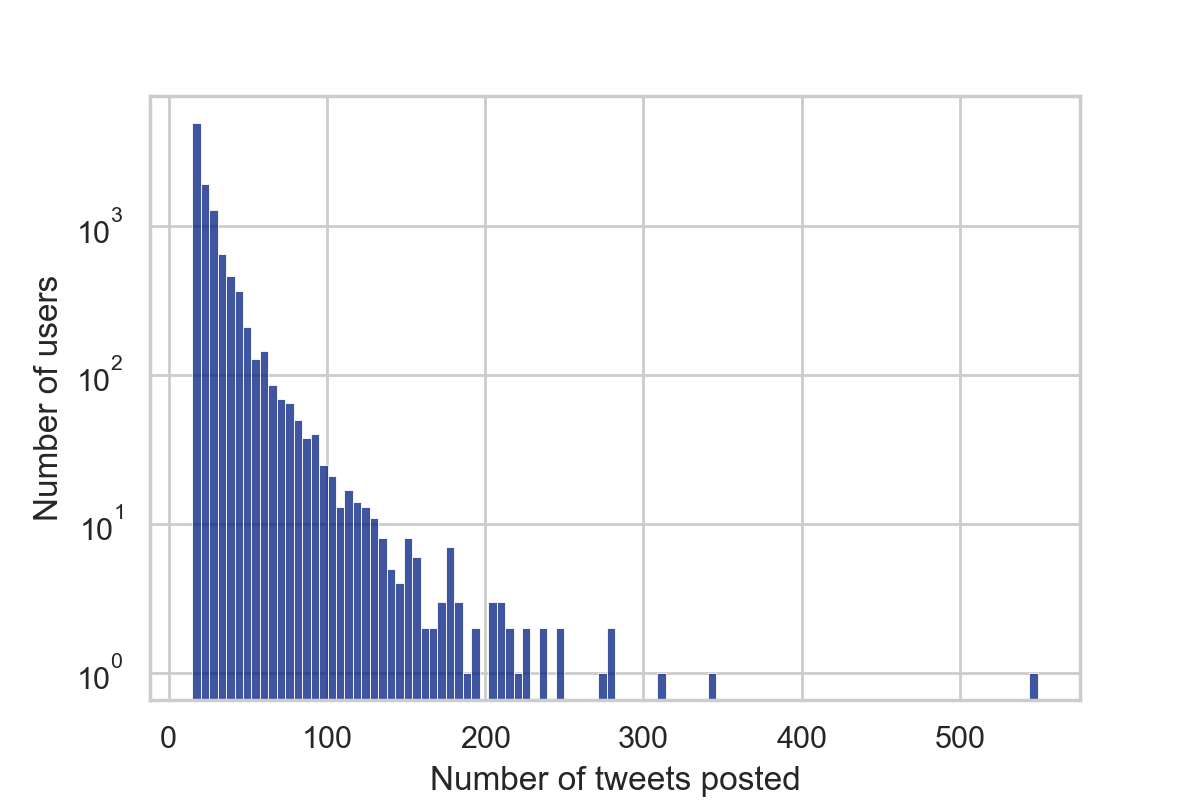
\includegraphics[width=0.5\textwidth]{user_per_tweet}
    \caption[Histogram of users per tweets]{Histogram representing the number of users per number of tweets}
    \label{fig:user_per_tweet}
\end{figure}
Analysing the user average sentiment distribution (figure \ref{fig:average_user_sentiment}), it is possible to notice that there are many users whose tweets are almost exclusively positive.
\begin{figure}
    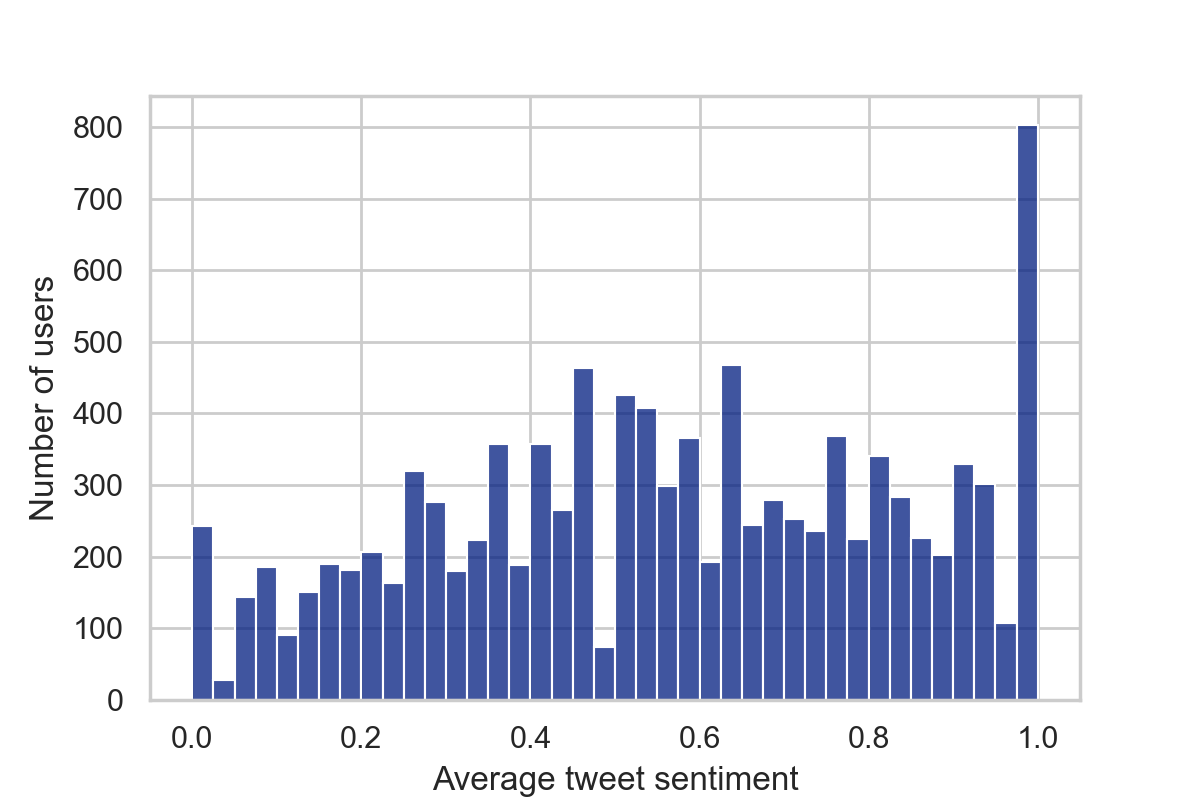
\includegraphics[width=0.5\textwidth]{average_user_sentiment}
    \caption[User average sentiment]{Histogram representing the number of users per average sentiment}
    \label{fig:average_user_sentiment}
\end{figure}
This odd behaviour led to a deeper investigation of the texts written by each user; a mean cosine similarity among the tweets posted by the same user was computed (figure \ref{fig:internal_similarity_users}), and it showed that a small but significant group of users
\begin{figure}
    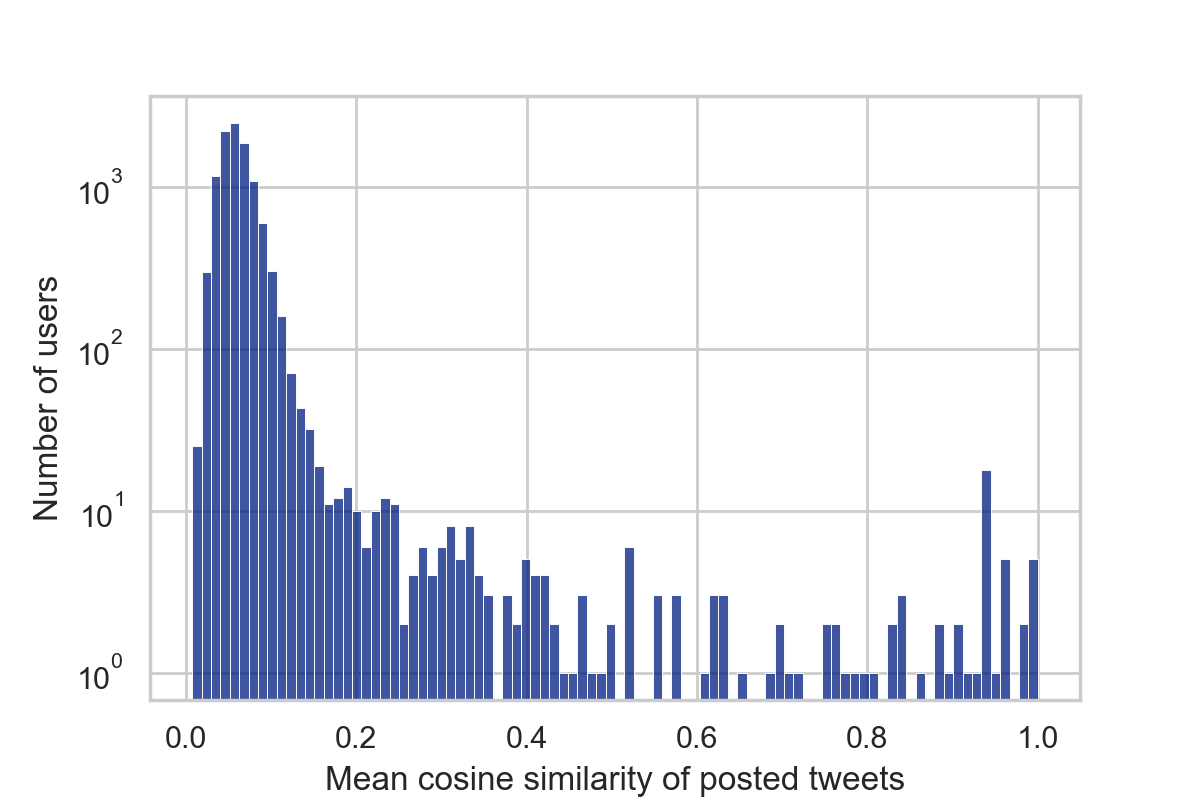
\includegraphics[width=0.5\textwidth]{internal_similarity_users}
    \caption[Mean cosine similarity]{Histogram representing the number of users per mean cosine similarity computed on the posted tweets of each user}
    \label{fig:internal_similarity_users}
\end{figure}



\section{Proposed approach}
In this section, you will present your solution. Please fill in accordingly.

You can use citations as follows: \cite{goodfellow2016deep} (you can add BibTeX citations in the \textit{bibliography.bib} file).

\subsection{Preprocessing}
\subsection{Model selection}
\subsection{Hyperparameters tuning}

\section{Results}
Here you will present your results (models \& configurations selected, performance achieved)

\section{Discussion}
Any relevant discussion goes here.

\bibliography{bibliography}
\bibliographystyle{ieeetr}

\end{document}
